\documentclass{beamer}

\mode<presentation> {
	\usetheme{Madrid}
}

\usepackage{graphicx}
\usepackage{booktabs}
\usepackage{cite}
\usepackage{tabularx}
\usepackage{csquotes}

\graphicspath{{images/}}

\title[Robotics \& Automation]{Evaluating Hierarchical Deep Learning Methods For Vision Based Robot Manipulation Of Dynamic Objects In Unstructured Environments}

\author[CET]{
	Department for Interdisciplinary Research\\ College of Engineering Trivandrum
}

\begin{document}
	
	\begin{frame}
		\maketitle
		
		\begin{tabularx}{\textwidth}{lXl}
			\textbf{Guided by,} & & \textbf{Presented by,} \\
			Linu Shine & & Sreejith Krishnan R \\
			Electronics and Comm. Engg. & & Robotics \& Automation
		\end{tabularx}
	\end{frame}
	
	\section{Motivation}
	
	\begin{frame}
		\frametitle{Motivation}
		Why robot manipulation?
		
		\begin{itemize}
			\item In order to assist in general tasks, autonomous robots should be able to interact with dynamic
			objects in unstructured environments
			
			\item Designing machines that can grasp and manipulate objects with anything approaching human levels of dexterity is first on the to-do list for robotics \cite{graspstate}
		\end{itemize}
		
		Hierarchical reinforcement learning allows to,
		
		\begin{itemize}
			\item Decompose complex task into hierarchy of sub-tasks
			\item Reuse sub-tasks in similar domain
			\item DNA for artificial intelligent agents
		\end{itemize}
	
		\begin{center}
			\textquote[Satinder Singh]{
				Stop learning tasks, start learning skills
			}
		\end{center}
	\end{frame}

	\section{Literature Survey}
	
	\begin{frame}[allowframebreaks]
		\frametitle{Literature survey}
		
		\begin{tabular}{m{2.25cm} | m{9cm}}
			\hline
			
			\textbf{Title} &
			Learning ambidextrous robot grasping policies \cite{dexnet4} - Science Robotics - 2019 \\
			\hline
			
			\textbf{Methodology} &
			Learns policies on synthetic training datasets generated using analytic models and domain randomization over a diverse range of objects, cameras, and parameters of physics for robust transfer from simulation to reality \\
			\hline
			
			\textbf{Merits} &
			\begin{itemize}
				\item Current state of the art in object picking
				\item 95\% success rate in real robot
				\item 300 mean pick per hour
			\end{itemize} \\
			\hline
		
			\textbf{Demerits} &
			\begin{itemize}
				\item Only for object picking
			\end{itemize}\\
			\hline
			
		\end{tabular}
	
		\begin{tabular}{m{2.25cm} | m{9cm}}
			\hline
			
			\textbf{Title} &
			Comparing Task Simplifications to Learn Closed-Loop Object Picking Using Deep Reinforcement Learning \cite{tasksimplification} - IEEE Robotics and Automation Letters - 2019\\
			\hline
			
			\textbf{Methodology} &
			Uses autoencoder to reduce dimensionality of camera data which is given to 3 layer CNN to get a low dimensional encoding. This encoding is used by a 2 layer feed-forward neural network to predict the optimum action. Uses RL to train the mentioned networks\\
			\hline
			
			\textbf{Merits} &
			\begin{itemize}
				\item No hand labeled data required
			\end{itemize} \\
			\hline
			
			\textbf{Demerits} &
			\begin{itemize}
				\item Low success rate (78\%) for manipulation of objects in clutter by real robot
				\item Non modular. Difficult to reuse model for similar task
			\end{itemize}\\
			\hline
			
		\end{tabular}
	
		\begin{tabular}{m{2.25cm} | m{9cm}}
			\hline
			
			\textbf{Title} &
			Regularized Hierarchical Policies for Compositional Transfer in Robotics \cite{rhpo} - DeepMind - 2019\\
			\hline
			
			\textbf{Methodology} &
			Use hierarchical modular policies for continuous control. \\
			\hline
			
			\textbf{Merits} &
			\begin{itemize}
				\item Best sample efficiency on both simulated and real robot
				\item Uses MPO optimization algorithm which reduces the number of hyperparameters
			\end{itemize} \\
			\hline
			
			\textbf{Demerits} &
			\begin{itemize}
				\item High level tasks are not automatically decomposed to sub tasks
				\item Low level policy is shared across all low level tasks making interpretability complicated
				\item Transferring specific skills from sub-tasks policy in a predictable manner is difficult
				\item Experiment results are obtained using model whose inputs include pose of objects in workspace
			\end{itemize}\\
			\hline
			
		\end{tabular}
	\end{frame}
	
	\section{Research Gap}
	\begin{frame}
		\frametitle{Research Gap}
		\begin{itemize}
			\item Low success rate on real world
			\item High training time due to low data efficiency
			\item Difficult to apply skills learned from one task to similar tasks
		\end{itemize}
	\end{frame}

	\section{Objectives}
	
	\begin{frame}
		\frametitle{Objectives}
		\begin{block}{Phase 1}
			\begin{itemize}
				\item Evaluate HRL for table clearing task on simulated environment
				\item Apply learned policies from simulated to real environment. Explore strategies to close the gap between success rate in simulation and real world
			\end{itemize}
		\end{block}
		
		\begin{block}{Phase 2}
			\begin{itemize}
				\item Explore methods to interpret skills learned by HRL
				\item Evaluate reusability of skills learned from table clearing task to similar tasks. Explore strategies for optimum reusability
				\item Explore strategies to improve mean picks per hour
			\end{itemize}
		\end{block}
	\end{frame}

	\begin{frame}[allowframebreaks]
		\frametitle{Methodology}
		
		\begin{columns}[c]
			\column{0.5 \textwidth}
			\begin{itemize}
				\item Options framework, MAXQ and hDQN HRL methods are considered for evaluation
				\item Evaluation will be based on  success rate, mean picks per hour and training time
				\item Simulation environment will be created on Bullet Physics Simulator
				\item URDF model of ABB IRB 120 robot with 2 finger parallel gripper, table and objects should be provided to simulator
			\end{itemize}
			
			\column{0.5 \textwidth}
			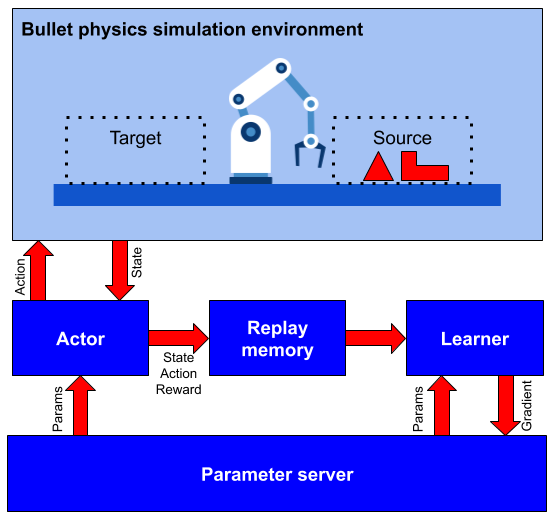
\includegraphics[width=6cm]{setup}
		\end{columns}
	

		\begin{itemize}
			\item 3D model of ABB IRB 120 robot is available. URDF file can be created using this models
			\item 3D CAD model of gripper of ABB IRB robot in robotics lab can be developed and URDF model can be created
			\item URDF database of 1000 random generated objects for robot grasping is available \cite{pdbrandom}
			\item ShapeNetSem \cite{shapenet2015}  contains 12,000 3D models spread across 270 object categories annotated with real-world dimensions and weight. URDF files can be automatically generated from 3D models
			\item Camera mounted on end effector of robot will give visual input to models. Learning phase will find the optimum action to take for the given visual input. Learned actions will be according to the value function tuned to optimize required parameters like manipulation time. Action will be of format $\begin{bmatrix}
			dx & dy & dz & d\alpha & d\beta & d\gamma & open\end{bmatrix}$. 
			\item GORILA architecture \cite{gorila} will be used to reduce training time. Simulator, actor, learner and parameter server will be separate processes interconnected by ZeroMQ \cite{zeromq} which can be distributed across multiple compute nodes.
			\item Preemptible VMs from Google Cloud \cite{gcppricing} (\$0.006655 / vCPU hour and \$0.000892 / GB hour) can be used as compute nodes. NVIDIA Tesla K80 with 12 GB RAM costs \$0.135 / hour can be used when GPU is more effective for computation (eg:- hDQN).
			\item Policies learned from simulator will be evaluated on ABB IRB 120 robot. Depth camera mounted on endeffector will provide visual feedback. Camera will be directly connected to computer. Program running in the computer will connect with robot via socket created in RAPID \cite{rapid} program running on robot controller. Robot and computer should be on same network. RAPID program will read actions send from computer, execute it and send feedback to computer.
		\end{itemize}
	\end{frame}

	\section{References}
	\begin{frame}[allowframebreaks]
		\frametitle{References}
		
		\bibliography{references}
		\bibliographystyle{unsrt}		
	\end{frame}
	
\end{document} 